\documentclass[border=3pt]{standalone}
\usepackage[T1]{fontenc}
\usepackage[utf8]{inputenc}
\usepackage{lmodern}
\usepackage{amsmath,amssymb}
\usepackage{xcolor}
\usepackage{tikz}
\usepackage{fontawesome5}
\usepackage{ragged2e}
\usetikzlibrary{shapes,shapes.geometric,shapes.misc,arrows.meta,positioning,
                calc,fit,backgrounds,decorations.pathreplacing,
                decorations.markings,patterns,chains}
\usetikzlibrary{decorations.pathreplacing,decorations.markings}
\definecolor{primary}{HTML}{1A5276}
\definecolor{secondary}{HTML}{2E86C1}
\definecolor{accent}{HTML}{E74C3C}
\definecolor{lightbg}{HTML}{EBF5FB}
\definecolor{defbg}{HTML}{FDF2E9}
\definecolor{greenhl}{HTML}{27AE60}
\definecolor{purplehl}{HTML}{8E44AD}
\definecolor{goldhl}{HTML}{B7950B}
\definecolor{tealhl}{HTML}{117A65}
\definecolor{codebg}{HTML}{F4F6F7}
\definecolor{neutral}{HTML}{707B7C}
\definecolor{dom1}{HTML}{1F618D}
\definecolor{dom2}{HTML}{117864}
\definecolor{dom3}{HTML}{6C3483}
\definecolor{dom4}{HTML}{922B21}
\definecolor{dom5}{HTML}{B7950B}
% --- carried over from ccna.sty so figures match the book exactly
\tikzset{
  dev/.style={rounded corners=3pt, draw=#1, fill=#1!8, text=#1!45!black,
              line width=0.9pt, minimum width=1.45cm, minimum height=1.05cm,
              align=center, font=\scriptsize\bfseries, inner sep=2pt},
  wirestyle/.style={line width=0.9pt, neutral!75},
  xconn/.style={line width=0.9pt, neutral!75, dash pattern=on 2.5pt off 2pt},
}

\newcommand{\Rtr}[3]{\node[dev=dom3] (#1) at #2 {\faIcon{route}\\#3};}
\newcommand{\Sw}[3]{\node[dev=dom2] (#1) at #2 {\faIcon{sitemap}\\#3};}
\newcommand{\Msw}[3]{\node[dev=dom3] (#1) at #2 {\faIcon{layer-group}\\#3};}
\newcommand{\Host}[3]{\node[dev=neutral] (#1) at #2 {\faIcon{desktop}\\#3};}
\newcommand{\Lap}[3]{\node[dev=neutral] (#1) at #2 {\faIcon{laptop}\\#3};}
\newcommand{\Srv}[3]{\node[dev=dom1] (#1) at #2 {\faIcon{server}\\#3};}
\newcommand{\Ap}[3]{\node[dev=dom5] (#1) at #2 {\faIcon{wifi}\\#3};}
\newcommand{\Wlc}[3]{\node[dev=dom5] (#1) at #2 {\faIcon{broadcast-tower}\\#3};}
\newcommand{\Fw}[3]{\node[dev=dom4] (#1) at #2 {\faIcon{shield-alt}\\#3};}
\newcommand{\Cld}[3]{\node[dev=neutral] (#1) at #2 {\faIcon{cloud}\\#3};}
\newcommand{\Phone}[3]{\node[dev=dom5] (#1) at #2 {\faIcon{phone-alt}\\#3};}
\newcommand{\Prn}[3]{\node[dev=neutral] (#1) at #2 {\faIcon{print}\\#3};}

% A link. The optional argument takes tikz options (e.g. xconn for a
% trunk drawn dashed); the fourth argument labels the link.
\newcommand{\wire}[4][wirestyle]{%
  \draw[#1] (#2) -- node[font=\tiny, text=neutral!85!black, fill=white,
                          inner sep=1.2pt, midway] {#4} (#3);}
\newcommand{\plainwire}[3][wirestyle]{\draw[#1] (#2) -- (#3);}


\newenvironment{topology}[1][]
  {\begin{center}\begin{tikzpicture}[font=\scriptsize,#1]}
  {\end{tikzpicture}\end{center}}


\newcommand{\cmd}[1]{\texttt{\small #1}}
\newcommand{\term}[1]{\textbf{\textcolor{primary}{#1}}}
\newcommand{\chref}[1]{Chapter~\ref{ch:#1}}
\newcommand{\ccnafitw}[1]{#1}
\providecommand{\thefigure}{}
% --- progressive builds
\newcount\buildlevel \buildlevel=99
% \stepvis{n}{..} appears from level n onward; \steponly{n}{..} at
% level n alone, which is how a caption is swapped rather than
% accumulated as the build advances.
\newcommand{\stepvis}[2]{\ifnum#1>\buildlevel\relax\else#2\fi}
\newcommand{\steponly}[2]{\ifnum#1=\buildlevel #2\fi}
\begin{document}
\begin{tikzpicture}[font=\scriptsize]
  \tikzset{
    dv/.style={rounded corners=3pt, draw=#1, fill=#1!8, text=#1!45!black,
               line width=0.9pt, minimum width=1.35cm, minimum height=0.95cm,
               align=center, font=\tiny\bfseries},
    w/.style={line width=0.85pt, neutral!65},
    hdr/.style={font=\scriptsize\bfseries, text=neutral!45!black}}

  % Every prose node gets an explicit text width. Without one the node is as
  % wide as its text, which both collides with its neighbours and drags the
  % picture's bounding box out sideways.
  \node[hdr, text width=13.5cm, align=center] at (5.3,3.5)
      {VLAN 30 must not reach the finance server --- but must still reach
       everything else};

  \node[dv=neutral] (h)   at (0,0.7)    {\faIcon{desktop}\\VLAN 30};
  \node[dv=dom3]    (r1)  at (3.0,0.7)  {\faIcon{route}\\R1};
  \node[dv=dom3]    (r2)  at (7.0,0.7)  {\faIcon{route}\\R2};
  \node[dv=dom1]    (fin) at (10.4,1.75){\faIcon{server}\\Finance};
  \node[dv=dom1]    (oth) at (10.4,-0.4){\faIcon{server}\\Everything\\else};
  \draw[w] (h) -- (r1);  \draw[w] (r1) -- (r2);
  \draw[w] (r2) -- (fin);  \draw[w] (r2) -- (oth);

  % wrong placement -- marker on the link, caption well below it
  \draw[accent!85, line width=1.4pt] (4.7,1.25) -- (5.3,0.15);
  \node[font=\tiny\bfseries, text=accent!75!black, align=center,
        text width=3.1cm, anchor=north] at (5.0,-0.35)
      {\faIcon{times-circle}~\textbf{standard} here\\blocks \emph{everything}};

  % right placement -- caption above, clear of the header
  \draw[dom2!80, line width=1.4pt] (8.5,2.0) -- (9.1,1.1);
  \node[font=\tiny\bfseries, text=dom2!45!black, align=center,
        text width=3.4cm, anchor=south] at (8.8,2.15)
      {\faIcon{check-circle}~\textbf{standard} here\\blocks only this server};

  \node[font=\tiny, text=neutral!85!black, align=center, text width=13.5cm]
      at (5.3,-1.85)
      {A standard ACL sees only \emph{who sent it}, so near the source it cannot
       tell the two servers apart. An \textbf{extended} ACL names the destination
       too, so it is safe at the source --- and saves carrying doomed traffic
       across the network.};
\end{tikzpicture}
\end{document}
